\section{Proste zagadnienia 1D}

Przypomnienie. Równanie Schrödingera:

\begin{equation*}
    i \hbar \frac{\partial}{\partial t} \Psi(x, t) = - \left[ \frac{\hbar^2}{2m} \frac{\partial^2}{\partial x^2} + V(x) \right] \Psi(x, t)
\end{equation*}

Jest to fundamentalne równanie opisujące ewolucję funkcji falowej cząstki kwantowej w czasie i przestrzeni.
W przypadku potencjału niezależnego od czasu, rozwiązania można rozdzielić na część przestrzenną i czasową, co prowadzi do równania stacjonarnego:


\begin{equation*}
    V \neq V(t) \implies \Psi(x, t) = \psi(x) e^{-i \frac{E}{\hbar} t} \quad ; \quad \frac{- \hbar^2}{2m} \frac{\partial^2}{\partial x^2} \psi(x) + V(x) \psi(x) = E \psi(x)
\end{equation*}

Funkcja falowa $\Psi(x,t)$ nie opisuje cząstki jako punktu, lecz daje rozkład prawdopodobieństwa znalezienia jej w danym miejscu
i czasie, co wynika z interpretacji Borna: 


\begin{equation*}
    P(x, t) = \left| \Psi(x, t) \right|^2 = \left| \psi(x) \right|^2
\end{equation*}

Prąd prawdopodobieństwa $j(x,t)$ wyraża przepływ prawdopodobieństwa i jest związany z zachowaniem prawdopodobieństwa w czasie,
co jest kwantowym odpowiednikiem przepływu cząstek:
\begin{equation*}
    j(x, t) = \frac{\hbar}{2mi} \left( \Psi^*(x, t) \frac{\partial}{\partial x} \Psi(x, t) - \Psi(x, t) \frac{\partial}{\partial x} \Psi^*(x, t) \right)
    = \frac{\hbar}{2mi} \left( \Psi^*(x) \frac{\partial}{\partial x} \Psi - \Psi(x) \frac{\partial}{\partial x} \Psi^* \right)
\end{equation*}


\subsection{Swobodna cząstka (tzn. V = 0, potencjał wszędzie jest zerowy)}

Rozwiązanie równania Schrödingera dla swobodnej cząstki to fale płaskie o postaci $\Psi(x) = A e^{ikx} + B e^{-ikx}$, gdzie
$k$ jest wektorem falowym związanym z energią kinetyczną cząstki. Energia jest zawsze nieujemna, a funkcje falowe muszą być
ograniczone, co wymusza rzeczywiste wartości $k$.


\begin{equation*}
    - \frac{\hbar^2}{2m} \frac{\partial^2}{\partial x^2} \psi(x) = E \psi(x)
\end{equation*}

gdzie:
\begin{equation*}
    k = \frac{\sqrt{2mE}}{\hbar}
\end{equation*}
%
\begin{equation*}
    \psi(x) = A e^{ikx} + B e^{-ikx}
\end{equation*}

$ k \in \mathbb{R} $, bo inaczej mamy rozbieżne $\psi(x)$. \\
$ E >= 0 $, bo $ k = \frac{\sqrt{2mE}}{\hbar^2} $, a $ 2m > 0 $, $ \hbar > 0 $.

Natomiast $E$ wyraża się wzorem:
\begin{equation*}
    E = \frac{\hbar^2 k^2}{2m}
\end{equation*}

\subsubsection{Zagadnienie na liczbę własną operatora pędu}
Operator pędu $\hat{p}_x = - i \hbar \frac{\partial}{\partial x}$ ma funkcje własne postaci fal płaskich, a wartości własne
odpowiadają momentom pędu $\pm \hbar k$. To pokazuje dualizm falowo-korpuskularny: cząstka ma jednocześnie cechy fali i cząstki.

\begin{equation*}
    \hat{p}_x \psi(x) = p_x \psi(x)
\end{equation*}

\begin{equation*}
    \hat{p}_x \psi(x) = -i\hbar \frac{\partial}{\partial x} \psi(x)
\end{equation*}

$p_x$ to liczba własna operatora pędu.

Dostajemy:
\begin{equation*}
    \psi(x) = C e^{i p_x x / \hbar} \implies p_x = \pm \hbar k
\end{equation*}

\begin{equation*}
    \psi(x, t) = \left( A e^{ikx} + B e^{-ikx} \right) e^{-i \frac{E}{\hbar} t}
\end{equation*}

Ponieważ $w = \frac{E}{\hbar}$, to:
\begin{equation*}
    \psi(x, t) = A e^{i(kx - wt)} + B e^{-i(kx + wt)}
\end{equation*}

Dalej spojrzymy na różne przypadki: \\

\textbullet{$B = 0$}

\begin{equation*}
    \psi(x, t) = A e^{i(kx - wt)}
\end{equation*}

\begin{equation*}
    P(x, t) = \left| \psi \right|^2 = \left| A \right|^2
\end{equation*}

\begin{equation*}
    j = \frac{\hbar k}{m} \left| A \right|^2 = \frac{p}{m} \left| A \right|^2 = \nu \left| A \right|^2
\end{equation*}

Symbol $\nu$ oznacza prędkość. Gdy $B=0$, fala jest biegnąca w prawo, prąd prawdopodobieństwa jest dodatni, co oznacza przepływ
cząstek w tym kierunku. Prawdopodobieństwo znalezienia cząstki jest jednakowe w całej przestrzeni - cząstka jest całkowicie rozproszona \\

\textbullet{$A = 0$}
Analogicznie:
\begin{equation*}
    j = - \frac{\hbar k}{m} \left| B \right|^2 = - \nu \left| B \right|^2
\end{equation*}

Gdy $A=0$, fala biegnie w lewo, prąd jest ujemny, co odpowiada przepływowi w przeciwnym kierunku. \\

\newpage
\textbullet{$A = B$}

\begin{equation*}
    \psi(x, t) = A \left( e^{ikx} + e^{-ikx} \right) e^{-i w t} = C \cos(kx) e^{-i w t}
\end{equation*}
gdzie $C = 2A$. \\
Wynikiem jest:
\begin{equation*}
    x = \frac{\pm \frac{\pi}{2} + n \pi}{k}, n \in \mathbb{N} \implies \cos(kx) = 0
\end{equation*}

\begin{figure}[H]
    \centering
    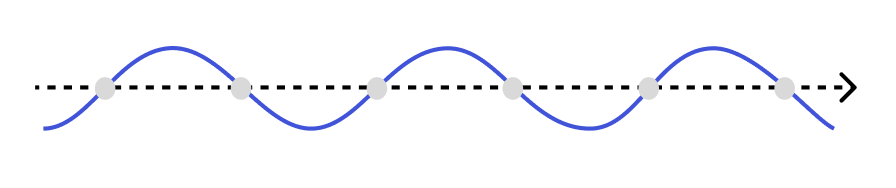
\includegraphics[width=0.5\textwidth]{fala-stojaca}
    \caption{Fala stojąca.}
    \label{fig:fala-stojaca}
\end{figure}

Gdy $A=B$ otrzymujemy węzły równomiernie rozmieszczone na osi $x$ - mamy falę stojącą (nieruchomą)
$\psi(x) \propto \cos(kx)$, gdzie prawdopodobieństwo jest nierównomiernie rozłożone i nie ma przepływu prądu. \\

\textbullet{$A \neq B$}

\begin{equation*}
    p(x) = \left| A \right|^2 + \left| B \right|^2 + \left( A B^* e^{i 2kx} + A^* B e^{-i 2kx} \right)
\end{equation*}

\begin{equation*}
    j = \nu \left( \left| A \right|^2 - \left| B \right|^2 \right)
\end{equation*}
Gdy $A \neq B$, fala jest superpozycją biegnących fal, a prąd jest różnicą ich natężeń, co oznacza przepływ prawdopodobieństwa w kierunku dominującej składowej.
Strumień będzie albo w jednym, albo w drugim kierunku. Zależnie czy większe jest $A$ czy $B$. \\




\subsection{Potencjał schodkowy}

Potencjał schodkowy to jedno z najprostszych i najważniejszych zagadnień w mechanice kwantowej, ilustrujące zachowanie
cząstki napotykającej nagłą zmianę potencjału. Model ten jest podstawą do zrozumienia zjawisk takich jak odbicie i
przejście cząstek na granicy różnych obszarów potencjału.

\begin{figure}[H]
    \centering
    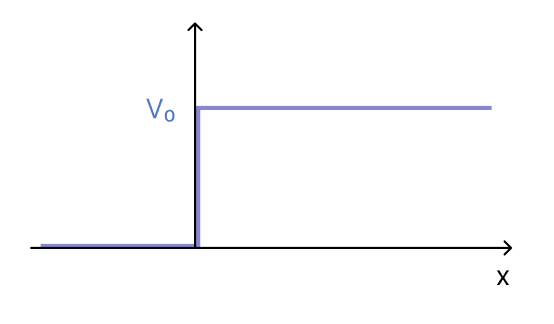
\includegraphics[width=0.5\textwidth]{potencjal-schodkowy}
    \caption{Potencjał schodkowy.}
    \label{fig:potencjal-schodkowy}
\end{figure}



\begin{equation*}
    v(x) = 
    \begin{cases}
        0, & x < 0 \\
        V_0, & x \geq 0
    \end{cases}
\end{equation*}

Rozważmy trzy podstawowe przypadki energii cząstki względem wysokości schodka: $E<0$, $0<E<V_0$ oraz $E>V_0$.

\textbullet{ $E < 0$}

Brak rozwiązań (bo $\frac{\partial^2}{\partial x^2} \psi(x) = \text{const}, \forall x \in \mathbb{R}$). \\
Dla energii ujemnej nie istnieją fizyczne rozwiązania równania Schrödingera w całej przestrzeni,
ponieważ wówczas druga pochodna funkcji falowej byłaby stała, co prowadzi do rozwiązań nielokalizowanych i
nieakceptowalnych fizycznie. Innymi słowy, nie ma dopuszczalnych stanów o ujemnej energii dla swobodnej cząstki w tym modelu.

\textbullet{ $0 < E < V_0$}

Dla $x < 0$:
\begin{equation*}
\frac{\partial^2}{\partial x^2} \psi(x) + k^2 \psi(x) = 0
\end{equation*}
%
\begin{equation*}
k = \left( \frac{2m}{h^2} E \right)^{1/2}
\end{equation*}


Dla $x<0$ cząstka zachowuje się jak swobodna fala o energii $E$, natomiast dla $x>0$,
gdzie potencjał jest wyższy niż energia, funkcja falowa ma charakter wykładniczo malejący. \\

Dla $x > 0$:
\begin{equation*}
\frac{\partial^2}{\partial x^2} \psi(x) - 2 \kappa^2 \psi(x) = 0
\end{equation*}
%
\begin{equation*}
\kappa = \left( \frac{2m}{h^2} (V_0 - E) \right)^{1/2}
\end{equation*}




Zatem dostajemy:
\begin{equation*}
\psi(x) = 
\begin{cases}
    A e^{ikx} + B e^{-ikx}, & x < 0 \\
    C e^{\kappa x} + D e^{-\kappa x} \implies \psi(x) = D e^{-\kappa x}, & x > 0
\end{cases}
\end{equation*}

W obszarze, gdzie energia jest mniejsza od potencjału, funkcja falowa w obszarze $x>0$ maleje wykładniczo,
co oznacza, że cząstka ma niezerowe, choć malejące prawdopodobieństwo znalezienia się w obszarze potencjału
wyższego niż jej energia - jest to efekt tunelowania kwantowego. \\

Jaki jest związek między wszystkimi współczynnikami? Zobaczmy. Szukamy warunków ciągłości.

\begin{equation*}
\psi(x) \in X(-\infty, \infty) \implies \text{dla } x = 0: A e^0 + B e^0 = D e^0 \implies A + B = D
\end{equation*}

\begin{equation*}
\frac{\partial}{\partial x} \psi(x) \in X(-\infty, \infty) \implies \text{dla } x = 0: i k (A - B) = - \kappa D
\end{equation*}

Warunki ciągłości funkcji falowej i jej pochodnej na granicy $x=0$ pozwalają wyznaczyć relacje między amplitudami fal odbitych i transmitowanych. \\

Dostajemy:
\begin{equation*}
\begin{cases}
    A = \frac{1 + i \kappa / k}{2} D \\
    B = \frac{1 - i \kappa / k}{2} D
\end{cases}
\end{equation*}

Zatem:
\begin{equation*}
\frac{B}{A} = e^{i \alpha} \implies \alpha =2 \arctan \left( - \left(  \frac{\nu_0}{E} - 1 \right) ^{1/2} \right)
\end{equation*}

Fala odbita różni się od fali padającej przesunięciem fazowym $\alpha$, co wpływa na interferencję i kształt fali stojącej w obszarze $x<0$.

Otrzymujemy:
\begin{equation*}
\psi(x) = 
\begin{cases}
    2 A e^{\frac{i \alpha}{2}} cos(kx - \frac{\alpha}{2}), & x < 0 \\
    2 A e^{\frac{i \alpha}{2}} cos(\frac{\alpha}{2} e^{-\kappa x}), & x > 0
\end{cases}
\end{equation*}

\begin{figure}[H]
    \centering
    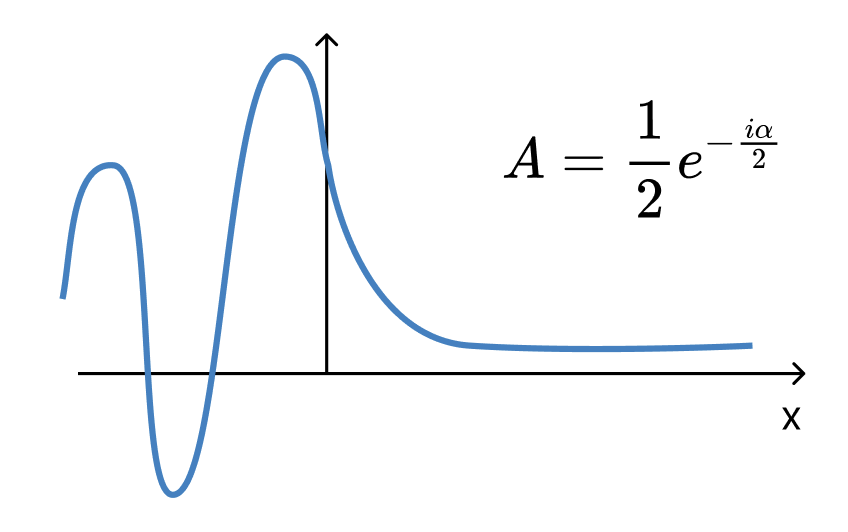
\includegraphics[width=0.5\textwidth]{fala-schodka}
    \label{fig:fala-schodka}
\end{figure}

Gdy wysokość schodka dąży do nieskończoności, to ogon jest jak "L".

Współczynnik odbicia:
\begin{equation*}
\frac{j_B}{j_A} = \frac{\nu \left| B \right|^2}{\nu \left| A \right|^2} = \frac{\left| B \right|^2}{\left| A \right|^2} = \left| e^{i \alpha} \right|^2 = 1
\end{equation*}
A więc wszystko się odbija. Mamy całkowite odbicie od schodka i nie ma przenikania do obszaru o wyższym potencjale. \\

Przypomniając wzór na $\kappa$, $\kappa = \left( \frac{2m}{h^2} (V_0 - E) \right)^{1/2}$, możemy zauważyć, że gdy $\kappa$ jest duża,
to spadek potencjału nie będzie mocny. Duża wartość $\kappa$ oznacza szybki spadek funkcji falowej w obszarze $x>0$,
co odpowiada silnemu tłumieniu prawdopodobieństwa znalezienia cząstki za barierą.


\textbullet{Rozważmy sytuację, gdy potencjał $V_0$ dąży do nieskończoności.}
W granicy $V_0 \to \infty$ bariera staje się nieprzenikalna, a funkcja falowa w obszarze $x>0$ zanika całkowicie.

Wtedy $\kappa$ dąży do nieskończoności:
\begin{equation*}
    \lim_{V_0 \to \infty} \frac{B}{A} = -1 \\
    \lim_{V_0 \to \infty} \frac{D}{A} = 0 \\
    \kappa \to \infty
\end{equation*}

\textbullet{Co będzie gdy potencjał $V_0$ jest skończony, a energia większa od potencjału?}
Dla energii większej niż potencjał, fala w obszarze $x>0$ ma charakter biegnący,
co oznacza możliwość przejścia cząstki przez barierę z pewnym prawdopodobieństwem.

\begin{equation*}
    \begin{cases}
        \psi = A e^{ikx} + B e^{-ikx}, & x < 0 \\
        \psi = C e^{ikx} + D e^{-ikx} = C e^{ikx}, & x > 0
    \end{cases}
\end{equation*}

Otrzymujemy:
\begin{equation*}
    \left\{
    \begin{aligned}
        & \frac{B}{A} = \frac{k - k'}{k + k'} \\
        & \frac{C}{A} = \frac{2k}{k + k'}
    \end{aligned}
    \right.
    \quad
    j = 
    \begin{cases}
        \nu \left( |A|^2 - |B|^2 \right), & x < 0 \\
        \nu' |C|^2, & x > 0
    \end{cases}
\end{equation*}

Gdzie $\nu$ oraz $\nu'$ wyrażają się następująco:
\begin{equation*}
    \nu = \frac{\hbar k}{m} = \frac{p}{m} \\
    \nu' = \frac{\hbar k'}{m}
\end{equation*}

Możemy zatem zapisać:
\begin{equation*}
    \frac{\left| B \right|^2}{\left| A \right|^2} + \frac{\nu'}{\nu} \frac{\left| C \right|^2}{\left| A \right|^2} = 1
\end{equation*}

Stąd:
\begin{equation*}
    \nu' \left| C \right| ^2 = \nu \left( \left| A \right| ^2 - \left| B \right| ^2 \right)
\end{equation*}

A więc prąd gęstości prawdopodobieństwa jest wszędzie taki sam. \\

Możemy wyznaczyć współczynnik odbicia R oraz przejścia T:
\begin{equation*}
    R = \frac{\left| B \right|^2}{\left| A \right|^2} = \left( \frac{1 - \sqrt{1 - \frac{V_0}{E}}}{1 + \sqrt{1 - \frac{V_0}{E}}} \right)^2
\end{equation*}

\begin{equation*}
    T = \frac{\nu' \left| C \right| ^2}{\nu \left| A \right| ^2} = \frac{4 \sqrt{1 - V_0/E}}{\left( 1 + \sqrt{1 - V_0/E} \right)^2}
\end{equation*}

Współczynnik odbicia $R$ oraz współczynnik przejścia $T$ dają w sumie 1:
\begin{equation*}
    R + T = 1
\end{equation*}



\subsection{Bariera potencjału}

\begin{figure}[H]
    \centering
    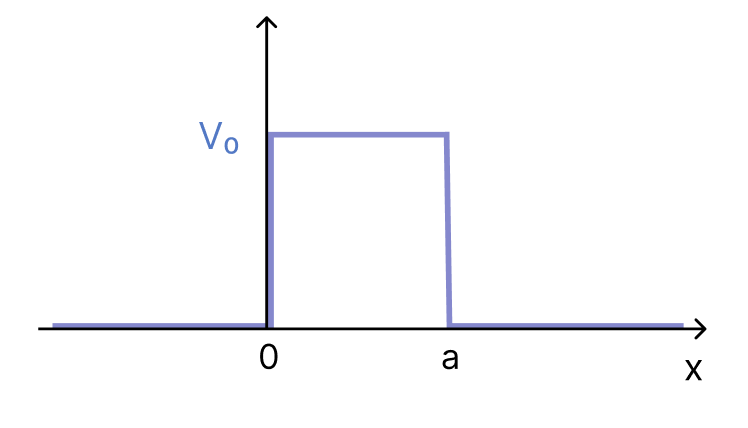
\includegraphics[width=0.5\textwidth]{bariera-potencjalu}
    \caption{Bariera potencjału.}
    \label{fig:bariera-potencjalu}
\end{figure}

\begin{equation*}
    V(x) = 
    \begin{cases}
        0, & x < 0 \\
        V_0, & 0 < x < a \\
        0, & x > a
    \end{cases}
\end{equation*}

Chcemy zrozumieć, jaka część fali przechodzi przez barierę potencjału, a jaka się odbija.
Zjawisko to jest kluczowe w mechanice kwantowej i nie ma klasycznego odpowiednika - nawet gdy energia cząstki
jest mniejsza niż wysokość bariery, istnieje niezerowe prawdopodobieństwo przejścia przez nią.

\textbullet{ $E < V_0$}



\begin{equation*}
    \psi(x) =
    \begin{cases}
        A e^{ikx} + B e^{-ikx}, & x < 0 \\
        C e^{ikx}, & x > a \\
        F e^{\kappa x} + G e^{-\kappa x}, & 0 < x < a
    \end{cases}
\end{equation*}

W obszarze bariery (0 < x < a) funkcja falowa ma charakter wykładniczy, co oznacza,
że fala jest tłumiona wewnątrz bariery, ale nie zanika natychmiastowo. \\

Definiujemy współczynnik przejścia $T$ oraz współczynnik odbicia $R$ analogicznie:
\begin{equation*}
    T = \frac{\left| C \right| ^2}{\left| A \right| ^2}
\end{equation*}

\begin{equation*}
    R = \frac{\left| B \right|^2}{\left| A \right|^2}
\end{equation*}

\newpage
Rozwiązujemy zgodnie z warunkami ciągłości:


\begin{equation*}
    \psi(x) \in C'(-\infty, \infty) \implies
    \left\{
    \begin{aligned}
      &\text{p. } x=0: \\
      &\quad A + B = F + G \\
      &\quad ik(A - B) = \kappa (F - G) \\[1.5ex]
      &\text{p. } x=a: \\
      &\quad C e^{ika} = F e^{\kappa a} + G e^{-\kappa a} \\
      &\quad ikC e^{ika} = \kappa (F e^{\kappa a} - G e^{-\kappa a})
    \end{aligned}
    \right.
    \implies
    \left\{
    \begin{aligned}
      &\frac{B}{A} = \frac{(k^2 + \kappa^2)(e^{\kappa a} - 1)}{e^{2\kappa a}(k + i\kappa)^2 - (k - i\kappa)^2} \\
      &\frac{C}{A} = \frac{h i k \kappa e^{-ika} - e^{\kappa a}}{e^{2\kappa a}(k + i\kappa)^2 - (k - i\kappa)^2}
    \end{aligned}
    \right.
\end{equation*}
%
\begin{equation*}
    \implies
    \begin{cases}
        R = ... = \left[ 1 + \frac{4 E (V_0 - E)}{V_0^2 \sin h^2(\kappa a)} \right] ^{-1} \\
        T = ... = \left[ 1 + \frac{V_0^2 \sin h^2(\kappa a)}{4 E (V_0 - E)} \right] ^{-1}
    \end{cases}
\end{equation*}

\begin{equation*}
    R + T = 1
\end{equation*}


Otrzymanych równań nie da się rozwiązać analitycznie, a więc rozwiązuje się je numerycznie. W mechanice kwantowej rozwiązania
numeryczne są bardzo (n razy) trudne. \\

\begin{figure}[H]
    \centering
    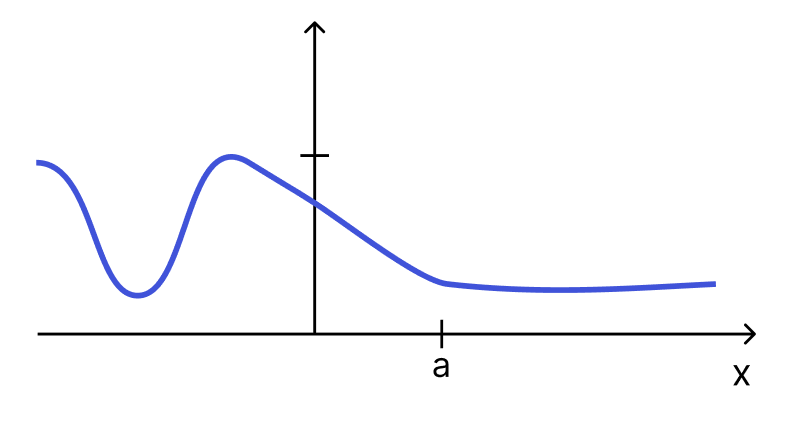
\includegraphics[width=0.5\textwidth]{czastka-przechodzi-przez-bariere}
    \caption{Cząstka przechodzi przez barierę.}
    \label{fig:czastka-przechodzi-przez-bariere}
\end{figure}


Na wykresie widzimy, że cząstka przechodzi przez barierę potencjału. Następuje tzw. "tunelowanie" cząstki przez barierę potencjału.
Tunelowanie kwantowe oznacza, że cząstka ma niezerowe prawdopodobieństwo znalezienia się po drugiej stronie bariery,
mimo że klasycznie byłoby to niemożliwe.\\

Uprośćmy teraz T. Dla $\kappa a >> 1$ zachodzi:
\begin{equation*}
    \sin h(\kappa a) \approx 1 / 2 e^{\kappa a} \implies T \approx \frac{16 E (V_0 - E)}{V_0^2} e^{- \kappa a}
\end{equation*}


Dla bariery o dużej szerokości lub wysokości prawdopodobieństwo przejścia spada wykładniczo z jej szerokością,
co wyjaśnia, dlaczego tunelowanie jest zjawiskiem subtelnym i silnie zależnym od parametrów bariery.
To wykładnicze tłumienie fali wewnątrz bariery jest kluczowe dla działania urządzeń takich jak mikroskop tunelowy
czy tranzystory tunelowe.\\


\textbullet{ $E > V_0$}
Gdy energia cząstki przekracza wysokość bariery, fala wewnątrz bariery ma charakter oscylacyjny,
co prowadzi do zjawiska interferencji i powstawania rezonansów.
\begin{equation*}
    0 < x < a: \psi = F e^{ik'x} + G e^{-ik'x}
\end{equation*}

Dla tego przypadku otrzumujemy następujące wzory na współczynniki odbicia $R$ oraz przejścia $T$:
\begin{equation*}
    R = \left[ 1 + \frac{4 E (E - V_0)}{V_0^2 \sin^2(k'a)} \right] ^{-1}
    T = \left[ 1 + \frac{V_0^2 \sin^2(k'a)}{4 E (E - V_0)} \right] ^{-1}
\end{equation*}

Warto zauważyć, że współczynniki te wykazują oscylacje w funkcji szerokości bariery, co odpowiada zjawisku rezonansowego przejścia fali. \\

\begin{figure}[H]
    \centering
    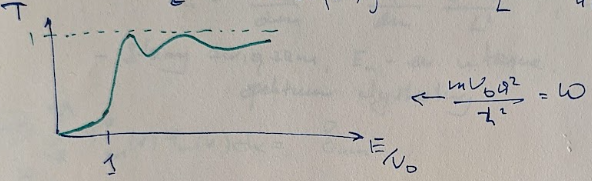
\includegraphics[width=0.5\textwidth]{wsp-przejscia}
    \label{fig:wsp-przejscia}
\end{figure}

Na wykresie widzimy, że mimo że mamy wysoką energię, mogą występować lokalne minima. \\


\subsubsection{Przykład: mikroskop tunelowy}
Zastosowanie tunelowania cząstek do badania struktury w mikroskopie tunelowym (skaningowym). (1979r.) \\

\begin{figure}[H]
    \centering
    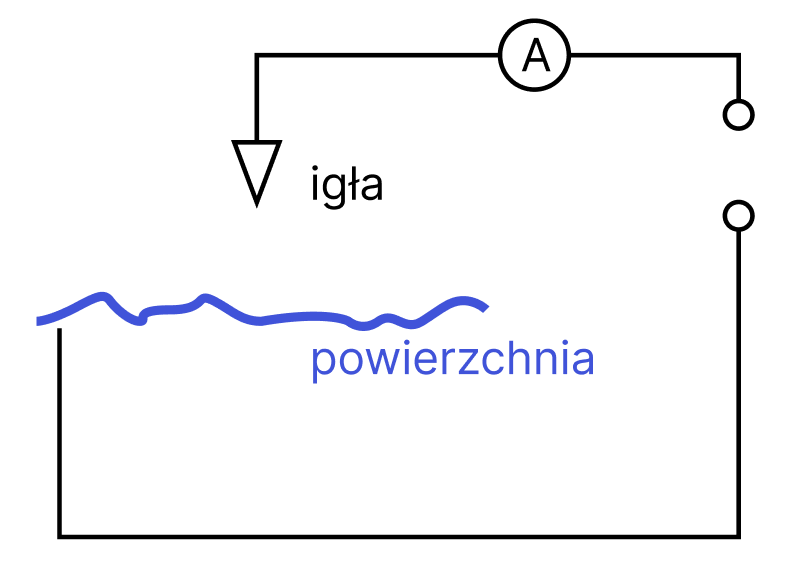
\includegraphics[width=0.5\textwidth]{mikroskop-tunelowy}
    \caption{Mikroskop tunelowy.}
    \label{fig:mikroskop-tunelowy}
\end{figure}

Mikroskop tunelowy wykorzystuje zjawisko tunelowania elektronów między ostrzem a badanym materiałem,
pozwalając na obrazowanie powierzchni z rozdzielczością atomową.

Gdy igła się porusza, zmienia się szerokość bariery. Energia jest stała, w zależności od położenia igły $V_0$ jest inne. Zatem zmienia się $T$,
a zatem zmienia się prąd. Zmiana szerokości bariery powoduje wykładniczą zmianę prawdopodobieństwa tunelowania, co przekłada się na zmiany
natężenia prądu tunelowego i pozwala na precyzyjne mapowanie topografii powierzchni.\\

Jak dokładne są te pomiary? Dokładność pomiarów mikroskopem tunelowym jest bardzo wysoka, ale wrażliwa na drgania i zakłócenia zewnętrzne,
które mogą zakłócić pomiar prądu tunelowego. Gdy tramwaj przejeżdza przez ulicę, zaburzy to wykonywane pomiary.



\subsection{Nieskończona kwadratowa studnia potencjału}

Nieskończona studnia potencjału to model idealizowany, w którym cząstka jest całkowicie uwięziona między nieprzekraczalnymi barierami potencjału.

\begin{figure}[H]
    \centering
    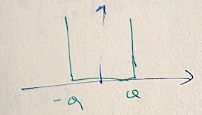
\includegraphics[width=0.5\textwidth]{nieskonczona-studnia-kwadratowa}
    \caption{Nieskończona studnia kwadratowa.}
    \label{fig:nieskonczona-studnia-kwadratowa}
\end{figure}

\begin{equation*}
    V(x) = 
    \begin{cases}
        0, & -a < x < a \\
        \infty, & |x| > a
    \end{cases}
\end{equation*}

Funkcja falowa musi zerować się na granicach studni i poza nią, ponieważ cząstka nie może znajdować się poza nieskończonymi barierami.

\begin{equation*}
    \psi(x) = 0, \quad \text{dla } |x| > a
\end{equation*}

Wewnątrz studni równanie Schrödingera opisuje swobodną cząstkę, ale z nałożonymi warunkami brzegowymi
wymuszającymi dyskretną strukturę stanów energetycznych

\begin{equation*}
    \text{Równanie Schrödingera: }
    \begin{cases}
        \frac{\hbar^2}{2m} \frac{\partial^2}{\partial x^2} \psi(x) = E \psi(x), & -a < x < a \\
        \psi(a) = 0, & \text{warunek brzegowy} \\
        \psi(-a) = 0, & \text{warunek brzegowy}
    \end{cases}
\end{equation*}
%
\begin{equation*}
    \implies
    \begin{cases}
        \psi(x) = A \cos(kx) + B \sin(kx), & -a < x < a \\
        k = \frac{\sqrt{2mE}}{\hbar^2}
    \end{cases}
\end{equation*}


Rozwiązanie jest kombinacją funkcji trygonometrycznych, które muszą spełniać warunki zerowania na brzegach studni.


\begin{equation*}
    \text{Warunki brzegowe: }
    \begin{cases}
        A \cos(ka) + B \sin(ka) = 0 \\
        A \cos(-ka) + B \sin(-ka) = 0
    \end{cases}
    \implies
    \begin{cases}
        A \cos(ka) = 0 \\
        B \sin(ka) = 0
    \end{cases}
\end{equation*}

Warunki te prowadzą do dwóch klas rozwiązań: parzystych (cosinusowych) i nieparzystych (sinusowych),
co odpowiada symetrii funkcji falowej względem środka studni.

Rozwiązujemy:
\begin{equation*}
    \begin{cases}
        B = 0 \\
        \cos(ka) = 0
    \end{cases}
    \implies
    \begin{cases}
        B = 0 \\
        ka = \frac{n \pi}{2 a} = \frac{n \pi}{L} = k_n, \quad n = 1, 3, 5, \ldots
    \end{cases}
\end{equation*}

Dla funkcji parzystych wartości $k_n$ są skwantowane, co prowadzi do dyskretnych poziomów energetycznych.


\begin{equation*}
    \psi_n(x) = A_n \cos(k_n x)
\end{equation*}

Normalizacja funkcji falowej zapewnia, że całkowite prawdopodobieństwo znalezienia cząstki w studni wynosi 1.

\begin{equation*}
    \int |\psi| dx = 1 \implies \int_{-\infty}^{\infty} A_n \cos^2 (k_n x) dx = 1 \implies A_n \sqrt{a} = 1 \implies A_n = \frac{1}{\sqrt{a}}
\end{equation*}


Następnie:

\begin{equation*}
    \begin{cases}
        A = 0 \\
        \sin(ka) = 0
    \end{cases}
    \implies
    \phi_n(x) = 1 \ \sqrt{a} \sin(\frac{n \pi}{2a} x), \quad n = 2, 4, 6, \ldots
\end{equation*}

Dla funkcji nieparzystych (sinusowych) również otrzymujemy skwantowane wartości $k_n$, co uzupełnia pełny zestaw stanów własnych.

Możemy zdefiniować własną bazę zagadnienia. \\
Energia stanów związanych (skwantowana, spektrum dyskretne), $E_n$ - ustalone wartości energii. \\

Spektrum energii jest dyskretne i rośnie z kwadratem liczby kwantowej $n$, co oznacza,
że cząstka może zajmować tylko określone poziomy energetyczne.

\begin{equation*}
    E_n = \frac{\hbar^2 k_n^2}{2m} = \frac{\hbar^2}{2m} \frac{n^2 \pi^2}{L^2}, \quad n = 1, 2, 3, \ldots
\end{equation*}


Gdzie $k_n$ jest związane z $E_n$ następująco:
\begin{equation*}
    k_n = \left( \frac{2 m}{\hbar ^2} E_n \right) ^{1/2}
\end{equation*}

Poziomy energetyczne zależą od szerokości studni $L=2a$ oraz masy cząstki, a minimalna energia jest większa niż zero, co jest efektem kwantowym.
Wartości $k_n$ są ściśle powiązane z poziomami energii i określają kształt funkcji falowej w studni. \\

\begin{figure}[H]
    \centering
    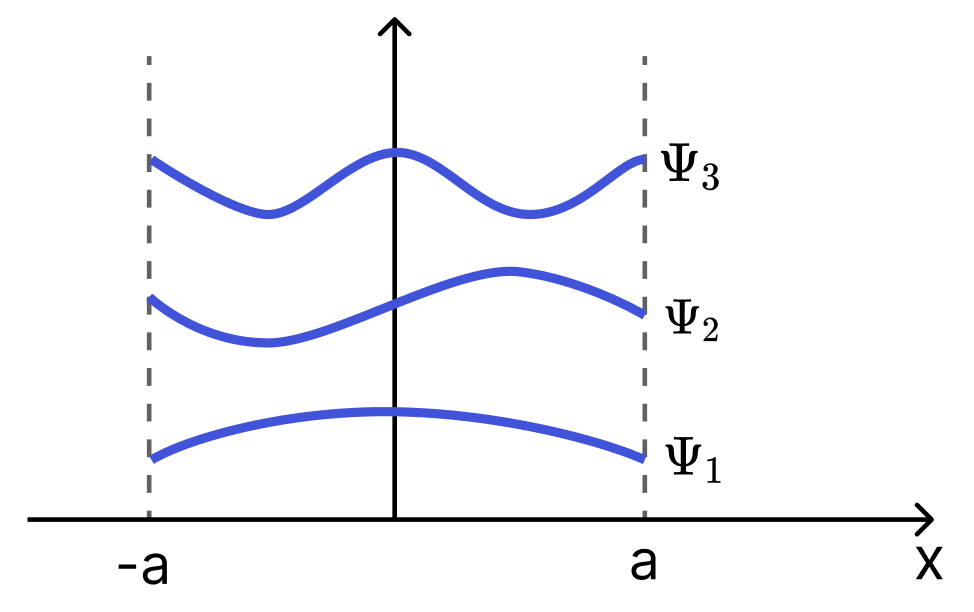
\includegraphics[width=0.5\textwidth]{studnia-kwadratowa-rozwiazanie}
    \caption{Poziomy energetyczne w nieskończonej studni potencjału.}
    \label{fig:studnia-kwadratowa-rozwiazanie}
\end{figure}

Wykres pokazuje dyskretne funkcje falowe cząstki w nieskończonej studni potencjału.
Każda krzywa odpowiada stanowi o określonej energii $E_n$. Liczba węzłów rośnie z numerem stanu,
a funkcje falowe są ograniczone do obszaru studni, zerując się na jej brzegach.


\subsection{Studnia kwantowa}

Studnia kwantowa o skończonej głębokości jest bardziej realistycznym modelem niż
studnia nieskończona – pozwala na częściowe „wyciekanie” funkcji falowej poza
obszar studni, czyli tunelowanie.

Wewnątrz studni potencjał jest stały i ujemny, a poza studnią równy zeru.
Cząstka o energii mniejszej niż zero jest związana z obszarem studni,
ale jej funkcja falowa nie zeruje się na brzegach, tylko zanika wykładniczo poza studnią.

\begin{equation*}
    V(x) = 
    \begin{cases}
        -V_0, & |x| < a \\
        0, & |x| > a
    \end{cases}
\end{equation*}

Mamy dwa przypadki - $E < 0$ oraz $E > 0$. \\
Dla $E < 0$ otrzymujemy stany związane (bound states), natomiast dla $E > 0$ – stany
rozproszone (scattering states).

\textbullet{ $E < 0$}

Pierwsze równanie dla $|x| < a$:

\begin{equation*}
    \frac{\partial^2}{\partial x^2} \psi(x) + \alpha^2 \psi(x) = 0
\end{equation*}

\begin{equation*}
    \alpha = \left( \frac{2m}{\hbar^2}(V_0 + E) \right)^{1/2} = \left( \frac{2m}{\hbar^2}(V_0 = |E|) \right)^{1/2}
\end{equation*}


Drugie równanie dla $x > a$:

\begin{equation*}
    \frac{\partial^2}{\partial x^2} \psi(x) - \beta^2 \psi = 0
\end{equation*}

\begin{equation*}
    \beta = \left( \frac{2m}{\hbar^2} E \right)^{1/2}
\end{equation*}

Rozważmy teraz dla $x > 0$:

\begin{equation*}
    \begin{cases}
        \psi_{\text{wewnętrzna}}(x) = A \cos(\alpha x), & 0 < x < a \\
        \psi_{\text{zewnętrzna}}(x) = C e^{-\beta x}, & x > a
    \end{cases}
\end{equation*}


\begin{equation*}
    \psi \in C'(-\infty, \infty) \implies
    \begin{cases}
        A \cos(\alpha a) = C e^{-\beta a} \\
        - \alpha A \sin(\alpha a) = - \beta C e^{-\beta a}
    \end{cases}
    \implies
    \alpha \tan(\alpha a) = \beta
\end{equation*}


Oraz

\begin{equation*}
    \begin{cases}
        \psi_{\text{wewnętrzna}}(x) = B \sin(\alpha x), & 0 < x < a \\
        \psi_{\text{zewnętrzna}}(x) = C e^{-\beta x}, & x > a
    \end{cases}
    \implies
    \alpha \cot(\alpha a) = -\beta
\end{equation*}


To daje nam dwa równania:


\[
\begin{cases}
    \xi = \alpha a \\
    \eta = \beta a
\end{cases}
\implies
\begin{cases}
    \xi \tan(\xi) = \eta \quad (1) \\
    \xi \cot(\xi) = -\eta \quad (2)
\end{cases}
\]

Równania te można rozwiązać graficznie lub numerycznie – liczba stanów
związanych zależy od głębokości i szerokości studni.


Własności:
\begin{itemize}
    \item $\xi^2 \eta^2 = \gamma^2$
    \item $\gamma = \sqrt{\frac{2mV_0 a^2}{\hbar^2}}$
\end{itemize}

Im większa głębokość lub szerokość studni, tym więcej stanów związanych może istnieć.

\begin{figure}[H]
    \centering
    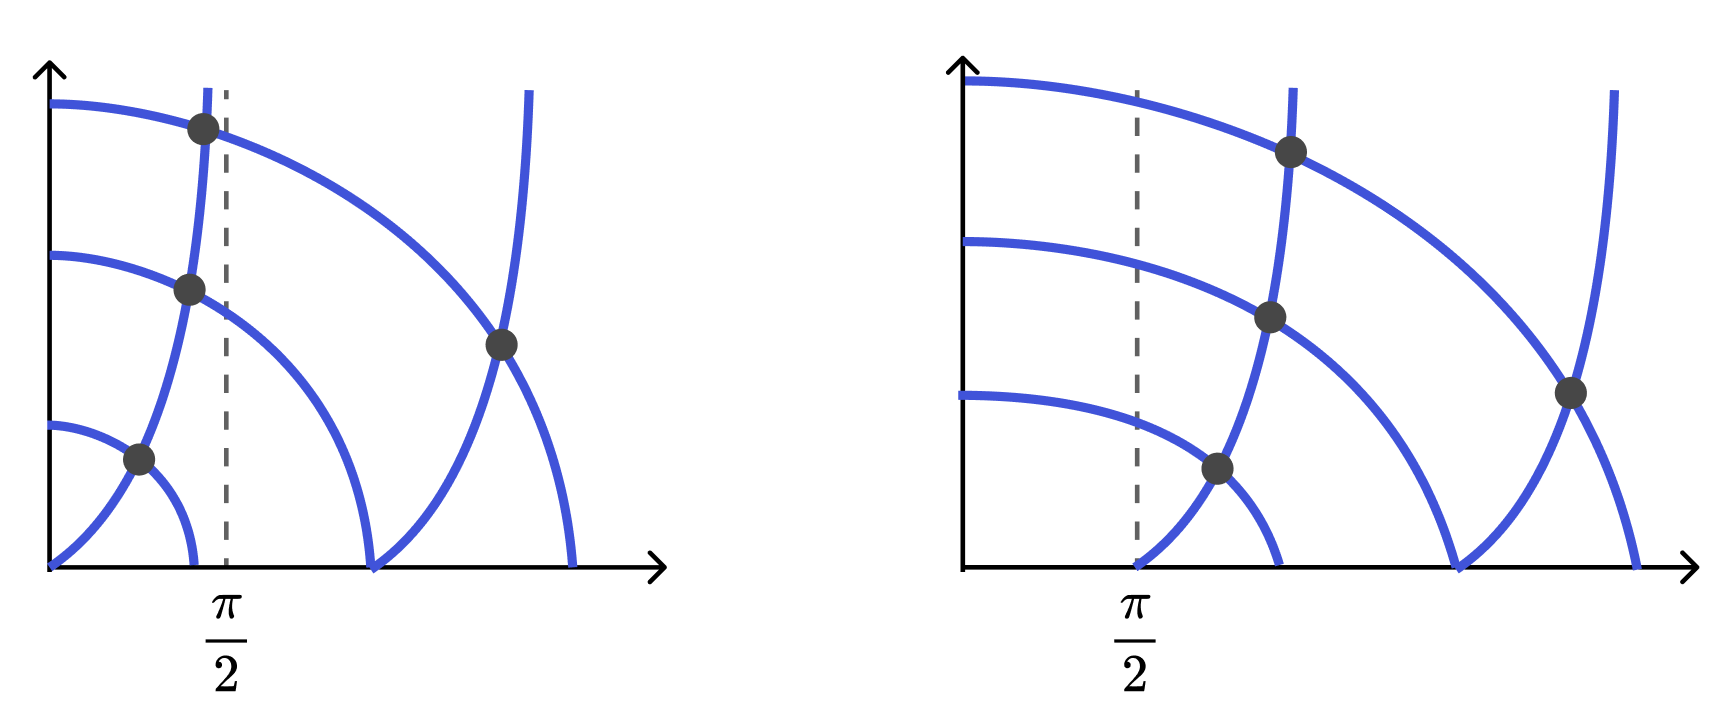
\includegraphics[width=0.5\textwidth]{studnia-rozw}
    \caption{Wykres po lewej odpowiada równaniu (1), a po prawej (2).}
    \label{fig:studnia-rozw}
\end{figure}

Węzły ukazują stany związane.

\textbullet{ $E > 0$}

Dla energii $E > 0$ rozwiązania opisują fale rozpraszane na studni – cząstka nie
jest już związana, lecz może przechodzić przez obszar studni z pewnym prawdopodobieństwem.


\begin{equation*}
    \begin{cases}
        \psi(x) =
        \begin{cases}
            A e^{ikx} + B e^{-ikx}, & x < -a \\
            C e^{ikx}, & x > a \\
            F e^{i\alpha x} + G e^{-i\alpha x}, & |x| < a
        \end{cases}
    \end{cases}
\end{equation*}

Gdzie:
\begin{itemize}
    \item $k = \left( \frac{2mE}{\hbar^2} \right)^{1/2}$
    \item $\alpha = \left( \frac{2m(E + V_0)}{\hbar^2} \right)^{1/2}$
\end{itemize}


Z tych równań otrzymujemy współczynniki odbicia i przejścia:

\begin{equation*}
    R = \left( 1 + \frac{4 E (V_0 + E)}{V_0^2 \sin^2(\alpha L)} \right) ^{-1}
\end{equation*}

\begin{equation*}
    T = \left( 1 + \frac{V_0^2 \sin^2(\alpha L)}{4 E (V_0 + E)} \right) ^{-1}
\end{equation*}

Współczynniki odbicia i przejścia określają prawdopodobieństwo odbicia i
transmisji cząstki przez studnię – ich suma zawsze wynosi 1.

\begin{figure}[H]
    \centering
    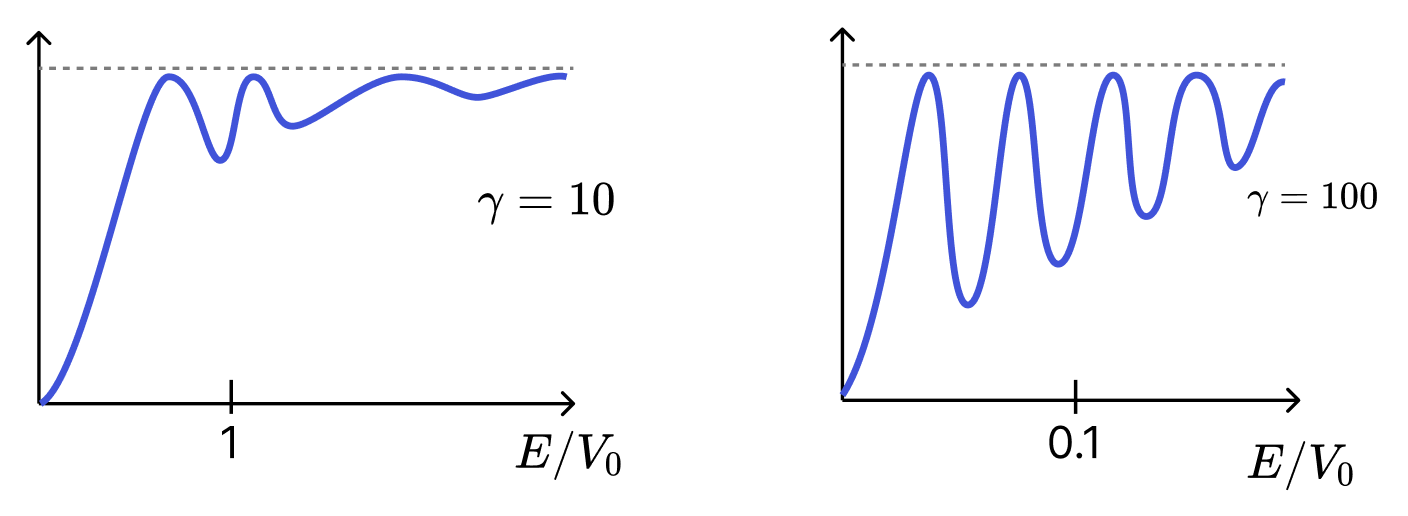
\includegraphics[width=0.5\textwidth]{studnia-rozw-2}
    \caption{Rozwiązania przy różnych $gamma$. Po prawej widać rezonanse.}
    \label{fig:studnia-rozw-2}
\end{figure}

Funkcje falowe opisują fale biegnące rozpraszane na studni, a współczynnik
przejścia wykazuje rezonanse – energie, dla których prawdopodobieństwo
przejścia przez studnię jest bliskie 1. Zjawisko to wynika z interferencji
falowej i prowadzi do lokalnych maksimów transmisji.
